\documentclass[tikz, border=10pt]{standalone}
\usetikzlibrary{shapes, arrows.meta, positioning, calc}

\begin{document}
	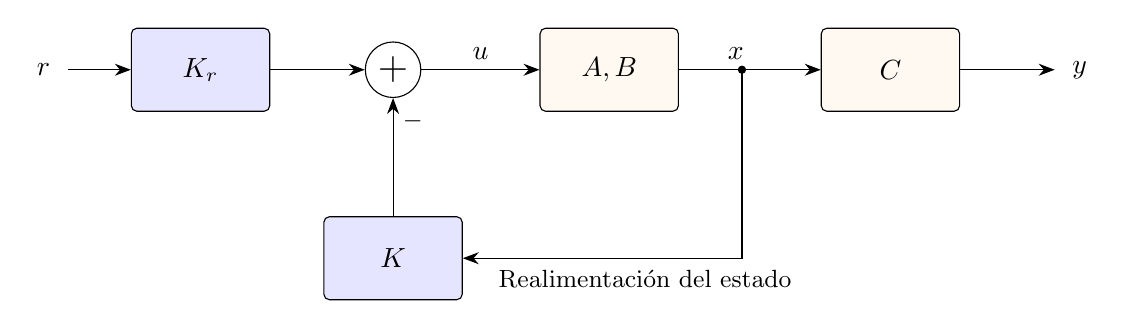
\begin{tikzpicture}[
		% Estilos ajustados para coincidir con la imagen del PFL
		block/.style = {draw, fill=blue!10, rectangle, minimum height=3em, minimum width=5em, align=center, rounded corners=2pt},
		proc_block/.style = {draw, fill=orange!5, rectangle, minimum height=3em, minimum width=5em, align=center, rounded corners=2pt},
		sum/.style = {draw, fill=white, circle, inner sep=2pt},
		input/.style = {coordinate},
		output/.style = {coordinate},
		node distance=2.5cm,
		>={Stealth[scale=1.2]}
		]
		
		% --- EJE PRINCIPAL ---
		\node [input] (r_in) {};
		\node [left=0.1cm of r_in] {$r$};
		
		% Bloque Kr
		\node [block, right=0.8cm of r_in] (kr) {$K_r$};
		
		% Sumador
		\node [sum, right=1.2cm of kr] (sum) {\Large +};
		
		% Bloques de la planta (Proceso)
		\node [proc_block, right=1.5cm of sum] (plant) {$A, B$};
		\node [proc_block, right=1.8cm of plant] (c_mat) {$C$};
		
		% Salida
		\node [output, right=1.2cm of c_mat] (salida) {};
		\node [right=0.1cm of salida] {$y$};
		
		% --- RAMA DE REALIMENTACIÓN ---
		\node [block, below=1.5cm of sum] (k_gain) {$K$};
		
		% --- CONEXIONES ---
		\draw [->] (r_in) -- (kr);
		\draw [->] (kr) -- (sum);
		\draw [->] (sum) -- node[above] {$u$} (plant);
		\draw [->] (plant) -- node[above, pos=0.4] (x_node) {$x$} (c_mat);
		\draw [->] (c_mat) -- (salida);
		
		% Punto de ramificación para x
		\coordinate (branch) at ($(plant.east) + (0.8,0)$);
		\fill (branch) circle (1.5pt);
		
		% Conexión de realimentación
		\draw [->] (branch) |- (k_gain);
		\draw [->] (k_gain.north) -| node[right, pos=0.9] {\small $-$} (sum);
		
		% Texto descriptivo abajo
		\node [below=-0.5cm of k_gain, xshift=3.2cm, font=\small] {Realimentación del estado};
		
	\end{tikzpicture}
\end{document}